%%
%% ACM FAccT format — sigconf, two-column
%% Ref: https://facctconference.org/authors/
%%
\documentclass[sigconf,review,anonymous]{acmart}
\AtBeginDocument{%
  \providecommand\BibTeX{{\scshape Bib\TeX}}}

%% ACM metadata — update for camera-ready
\setcopyright{acmlicensed}
\acmConference[FAccT '26]{ACM Conference on Fairness, Accountability, and Transparency}{2026}{Athens, Greece}
\acmYear{2026}
\acmDOI{XXXXXXX.XXXXXXX}
\acmISBN{978-1-4503-XXXX-X/26/06}

\citestyle{acmauthoryear}

\usepackage{amsmath}
\usepackage{amssymb}
\usepackage{booktabs}
\usepackage{xcolor}
\usepackage{multirow}


\definecolor{funcred}{HTML}{E63946}
\definecolor{contblue}{HTML}{457B9D}
\definecolor{siggreen}{HTML}{2D6A4F}

\newcommand{\tcd}{\text{TCD}}
\newcommand{\funcword}[1]{\texttt{#1}}
\newcommand{\pval}[1]{\ensuremath{p=#1}}

\title{Where Does Bias Hide? Token-Level Attribution Reveals Distributed Bias Propagation in Late-Interaction Retrieval}

\author{Chris Ziyu Kong}
\affiliation{%
  \institution{Brown University}
  \city{Providence}
  \state{Rhode Island}
  \country{USA}
}
\email{ziyukong@brown.edu}

\renewcommand{\shortauthors}{Kong}

%% CCS Concepts — required by ACM
\begin{CCSXML}
<ccs2012>
   <concept>
       <concept_id>10010147.10010178.10010187</concept_id>
       <concept_desc>Computing methodologies~Information extraction</concept_desc>
       <concept_significance>500</concept_significance>
   </concept>
   <concept>
       <concept_id>10010147.10010257.10010293.10010294</concept_id>
       <concept_desc>Computing methodologies~Neural networks</concept_desc>
       <concept_significance>500</concept_significance>
   </concept>
   <concept>
       <concept_id>10003456.10003462.10003561</concept_id>
       <concept_desc>Social and professional topics~User characteristics</concept_desc>
       <concept_significance>300</concept_significance>
   </concept>
</ccs2012>
\end{CCSXML}

\ccsdesc[500]{Computing methodologies~Information extraction}
\ccsdesc[500]{Computing methodologies~Neural networks}
\ccsdesc[300]{Social and professional topics~User characteristics}

\keywords{bias auditing, dense retrieval, ColBERT, fairness, tokenization, names}

\begin{document}
\maketitle

% ===========================================================================
\begin{abstract}
We present a mechanism-level audit of identity-related bias in ColBERT, a late-interaction dense retrieval model. Using ColBERT's decomposable MaxSim scoring, we introduce \emph{Token Contribution Disparity} (TCD), a metric that attributes bias to individual query tokens after counterfactual identity swaps. Across 43{,}065 controlled tests spanning 33 professions and 65 names, we find that: (1)~bias propagates primarily through function words (``is,'' ``who,'' ``a''), not through semantically relevant content words, at a ratio of \textbf{1.44$\times$}; (2)~rare names---those fragmented into more subword tokens by BPE---amplify this effect by up to \textbf{1.84$\times$}; (3)~the strongest confound-decomposition signals are cross-gender and tokenization mismatch, with a weaker residual race-category effect; (4)~the function-word propagation pattern holds at nearly identical magnitude (\textbf{1.42$\times$}, $p < 10^{-25}$) in naturalistic prose; and (5)~a BM25 control produces \emph{zero} function-word propagation, confirming this is a contextual-representation phenomenon. Together, these findings reveal that bias in transformer-based retrieval is distributed and context-mediated---not localized in lexical associations---with implications for both measurement and mitigation.
\end{abstract}

% ===========================================================================
\section{Introduction}
\label{sec:intro}

Search systems shape information access. Modern neural retrieval models---which encode queries and documents into dense vector representations and rank results by learned semantic similarity rather than exact keyword overlap---now underpin production search at scale. These systems determine what information users encounter first, influencing hiring decisions, research visibility, and access to services. When a retrieval model ranks documents about a person, the ranking implicitly distributes attention, visibility, and opportunity~\cite{singh2018}. If identity cues---names or pronouns---affect relevance scores, the system participates in discriminatory allocation even when no explicit demographic filter is applied.

Prior work has demonstrated that neural retrieval models produce measurably biased outputs~\cite{rekabsaz2021, ziems2024}, and that names alone can distort embedding similarity~\cite{manchanda2025}. However, these studies operate at the \emph{aggregate} level: they show \emph{that} systems are unfair without explaining the internal mechanism through which identity information changes relevance scores.

We pursue a different question: \textbf{where inside a neural retriever does identity-related bias actually reside, and how does it propagate to the output score?} This question matters because mechanism-level understanding enables qualitatively different responses. Without it, we cannot distinguish between a model that has learned stereotyped lexical associations (``nurse'' $\leftrightarrow$ ``female'') and one whose subword tokenizer systematically disadvantages unfamiliar names---two failure modes that require fundamentally different fixes. Aggregate-level audits conflate these causes. Moreover, if bias concentrates in a specific subset of token representations, targeted interventions can be scoped to those representations without degrading overall retrieval quality. And if the bias pathway runs through infrastructure components like the tokenizer, the finding generalizes beyond any single model to every system built on the same tokenization scheme.

ColBERT~\cite{khattab2020, santhanam2022} provides a unique opportunity to answer this question. Unlike single-vector bi-encoder models such as DPR~\cite{karpukhin2020}, which compress entire passages into a single dense vector, ColBERT's \emph{late-interaction} architecture preserves token-level document representations and computes relevance through fine-grained MaxSim matching. This means the total score can be decomposed into individual query-token contributions. By swapping identity markers in otherwise identical documents and observing which query tokens' contributions change, we can localize the pathways through which bias propagates.

Our contributions are:

\begin{enumerate}
\item \textbf{TCD metric.} We introduce Token Contribution Disparity, the first token-level bias attribution metric for dense retrieval (Section~\ref{sec:method}).

\item \textbf{Function-word bias propagation.} We show that bias flows through semantically vacuous function words (``is,'' ``who,'' ``a''), not through content words (``doctor,'' ``nurse''), overturning the intuition that bias equals lexical association (Section~\ref{sec:results:funcword}).

\item \textbf{Rarity amplification.} Rare names that fragment into more BPE tokens amplify bias by up to 1.84$\times$, revealing tokenization as a hidden fairness tax (Section~\ref{sec:results:rarity}).

\item \textbf{Confound decomposition.} A structured name-pair design isolates gender, tokenization, frequency, and race as bias drivers, finding composite rather than single-factor explanations (Section~\ref{sec:results:decomposition}).

\item \textbf{Ecological validation.} The core pattern generalizes from synthetic templates to naturalistic prose and is absent in BM25, confirming it is specific to contextual models (Section~\ref{sec:results:validation}).
\end{enumerate}


% ===========================================================================
\section{Related Work}
\label{sec:related}

\paragraph{Fairness in retrieval.}
Singh and Joachims~(\citeyear{singh2018}) formalized exposure fairness, showing that ranking systems distribute attention unevenly. Rekabsaz et al.~(\citeyear{rekabsaz2021}) measured gender bias in BERT-based rankers and proposed adversarial mitigation, but their analysis remains at the aggregate-ranking level. Krieg et al.~(\citeyear{krieg2023}) created the Grep-BiasIR dataset for gender representation bias. Our work differs by tracing bias to its \emph{internal} mechanism rather than its statistical summary.

\paragraph{Names as identity proxies.}
Bertrand and Mullainathan~(\citeyear{bertrand2004}) established name-swap audit methodology in their landmark resume experiment. Sweeney~(\citeyear{sweeney2013}) showed similar effects in online advertising. Caliskan et al.~(\citeyear{caliskan2017}) demonstrated with WEAT that static embeddings absorb human-like biases, and De-Arteaga et al.~(\citeyear{dearteaga2019}) showed stereotyped representations persist even when explicit gender markers are removed. Manchanda and Shivaswamy~(\citeyear{manchanda2025}) found that names distort embedding similarity in isolation. We adopt the name-swap framework but go beyond aggregate scores to analyze \emph{token-level} mechanisms.

\paragraph{Tokenization and representation.}
Bostrom and Durrett~(\citeyear{bostrom2020}) showed that subword tokenization choices affect downstream model behavior. Sennrich et al.~(\citeyear{sennrich2016}) introduced BPE for neural MT, which forms the basis of most modern tokenizers. Recent work has begun to connect tokenization disparities directly to fairness harms: Petrov et al.~(\citeyear{petrov2023}) demonstrated that multilingual BPE tokenizers introduce systematic cost and performance unfairness across languages, and Ovalle et al.~(\citeyear{ovalle2024}) showed that BPE over-fragmentation of data-scarce neopronouns is a direct cause of LLM misgendering. For retrieval, Goldfarb-Tarrant et al.~(\citeyear{goldfarb2024}) showed that identity-linked information remains encoded in dense retrieval representations. However, no prior work has empirically demonstrated that BPE fragmentation mediates bias \emph{magnitude} in retrieval scoring. We integrate tokenization into the bias story by providing this first empirical demonstration.

\paragraph{ColBERT and late interaction.}
ColBERT~\cite{khattab2020} and ColBERTv2~\cite{santhanam2022} are the only widely used retrievers that preserve per-token representations and compute scores via MaxSim. This makes them uniquely suited for token-level attribution, a property that single-vector models~\cite{karpukhin2020} fundamentally lack.


% ===========================================================================
\section{Methodology}
\label{sec:method}

\subsection{Retrieval Scenario and Definitions}

We study bias in \emph{candidate retrieval}---the task of ranking person-describing documents in response to a professional query (e.g., an employer searching ``Who is a qualified doctor?''). In our experiments:

\begin{itemize}
\item \textbf{Queries} are profession-oriented search queries drawn from a set of 33 professions (e.g., ``Who is a qualified software engineer?,'' ``Who is an experienced doctor?'').
\item \textbf{Documents} are short candidate descriptions generated from templates with an identity marker (name or pronoun) and professional credentials (e.g., ``Emily has over ten years of clinical experience'').
\end{itemize}

We study ColBERTv2~\cite{santhanam2022}, a late-interaction retrieval model. ColBERT independently encodes queries and documents into per-token L2-normalized embeddings using a shared BERT encoder with distinct input prefixes (\texttt{``query:~''} for queries, \texttt{``document:~''} for documents). Relevance is computed via \textbf{MaxSim}:
\begin{equation}
S(Q, D) = \sum_{i=1}^{|Q|} \max_{j \in [1,|D|]} \; \mathbf{q}_i^\top \mathbf{d}_j
\label{eq:maxsim}
\end{equation}
where $\mathbf{q}_i$ and $\mathbf{d}_j$ are the L2-normalized embeddings of the $i$-th query token and $j$-th document token, respectively.

\paragraph{Counterfactual design.} A \textbf{counterfactual pair} $(D_A, D_B)$ consists of two documents identical in every respect except for an identity marker (name or pronoun). For example:
\begin{quote}
$D_A$: ``Emily has over ten years of experience in this field.'' \\
$D_B$: ``Lakisha has over ten years of experience in this field.''
\end{quote}
The \emph{same query} $Q$ is scored against both documents. The per-token contribution of query token $q_i$ to each document is $c_i^A = \max_j \mathbf{q}_i^\top \mathbf{d}_j^A$ and $c_i^B = \max_j \mathbf{q}_i^\top \mathbf{d}_j^B$.

\paragraph{Validity of pairwise scoring.} A critical property of ColBERT's architecture is that $S(Q, D)$ is computed independently for each query--document pair: each document is encoded without knowledge of the query or other documents. Consequently, the scores $S(Q, D_A)$ and $S(Q, D_B)$ computed in our pairwise setting are \emph{mathematically identical} to the scores that would be assigned if $D_A$ and $D_B$ appeared alongside millions of other documents in a full retrieval index. This independence property---shared by all bi-encoder and late-interaction architectures---ensures that our pairwise comparisons faithfully reflect the model's scoring behavior in a production retrieval pipeline.

\subsection{Token Contribution Disparity (TCD)}

\begin{figure*}[t]
  \centering
  
\includegraphics[width=\textwidth]{figures/tcd_schematic.pdf}
  \caption{Overview of TCD computation. A query is matched against two documents differing only in an identity marker (Emily $\to$ Lakisha). ColBERT's MaxSim computes per-token contributions $c_i^A$ and $c_i^B$; TCD is the absolute difference. Function words (blue) show higher TCD than content words (orange), indicating identity information ``leaks'' through context-dependent tokens.}
  \label{fig:tcd_schematic}
\end{figure*}

We define the \textbf{Token Contribution Disparity} for query token $q_i$ as:
\begin{equation}
\tcd(q_i) = |c_i^A - c_i^B|
\label{eq:tcd}
\end{equation}

TCD measures how much a single query token's score contribution changes when the identity marker is swapped. Intuitively, a high TCD value means that a token's retrieval contribution is sensitive to the identity swap: the identity change in the document has ``leaked'' into that token's contextual representation and altered how it matches. When we say a token ``carries more bias,'' we mean its TCD is systematically higher---its score contribution shifts more when an identity marker is changed, even if the token itself (e.g., ``is'' or ``a'') has no semantic connection to the identity being tested.

 We classify each query token as \emph{function} (``is,'' ``who,'' ``a,'' etc.) or \emph{content} (``doctor,'' ``qualified,'' etc.) and compute aggregate metrics:
\begin{align}
\text{Func-TCD} &= \frac{1}{|\mathcal{F}|} \sum_{q_i \in \mathcal{F}} \tcd(q_i) \\
\text{Cont-TCD} &= \frac{1}{|\mathcal{C}|} \sum_{q_i \in \mathcal{C}} \tcd(q_i)
\end{align}

The \textbf{Score Sensitivity} (SS) normalizes the total score difference:
\begin{equation}
\text{SS} = \frac{|S(Q, D_A) - S(Q, D_B)|}{\frac{1}{2}(S(Q, D_A) + S(Q, D_B))}
\end{equation}

\subsection{Name Pool and Confound Decomposition}
\label{sec:method:names}

Our experiments use a curated pool of 65 names drawn from the Bertrand and Mullainathan~(\citeyear{bertrand2004}) audit set and expanded via the Rosenman et al.~(\citeyear{rosenman2023}) first-name ethnicity database. Each name is annotated with race, gender, BPE token count (verified against the ColBERTv2 tokenizer), and within-race frequency from the Rosenman prevalence tables.

To decompose confounded name effects, we construct five \emph{matched-pair families}:
\begin{itemize}
\item \textbf{Race}: same gender, token count, and frequency; vary race.
\item \textbf{Gender}: same race, token count, and frequency; vary gender.
\item \textbf{Tokenization}: same race, gender, and frequency; vary BPE token count.
\item \textbf{Frequency gap}: same race, gender, and token count; vary log-frequency gap.
\item \textbf{Absolute rarity}: same race, gender, token count, and near-equal frequency; median-split on mean log-frequency.
\end{itemize}

Statistical models use OLS with clustered standard errors at the pair level and profession and template fixed effects.

\subsection{Experimental Phases}

Our experiments proceed in five phases:

\begin{description}
\item[P0] \emph{Control validation}: 1{,}080 comparisons verifying that identity swaps produce larger function-word TCD than arbitrary non-identity substitutions ($p < 10^{-8}$, Cohen's $d = 0.37$).

\item[P1] \emph{Profession expansion}: 1{,}287 tests across 33 professions and three swap types (10 name pairs, 3 pronoun swaps) confirming function-word dominance at scale.

\item[P2/P2b] \emph{Name confound decomposition}: 43{,}065 tests (P2) plus a Rosenman-backed targeted validation (P2b) with 65 names and 124 race-family pairs.

\item[RT] \emph{Real-text validation}: 1{,}680 tests using 12 naturalistic passages spanning 7 text categories.

\item[BM25] \emph{Non-contextual control}: 1{,}400 tests using BM25 on the same passages and name pairs.
\end{description}


% ===========================================================================
\section{Results}
\label{sec:results}

% ------- 4.1 Function-Word Bias -------
\subsection{Function Words Carry More Bias Than Content Words}
\label{sec:results:funcword}

Across 1{,}287 P1 tests spanning 33 professions, function words consistently exhibit higher TCD than content words---that is, their MaxSim score contributions are more sensitive to identity swaps than those of semantically relevant content words:

\begin{table}[t]
\centering
\small
\begin{tabular}{lcccc}
\toprule
Token Type & $N$ & Mean $|\tcd|$ & Ratio & $p$ \\
\midrule
\textbf{Function} & --- & \textbf{0.0210} & \multirow{2}{*}{\textbf{1.44$\times$}} & \multirow{2}{*}{0.0002} \\
Content            & --- & 0.0146           &                                         & \\
\bottomrule
\end{tabular}
\caption{Function words carry 1.44$\times$ more bias (|TCD|) than content words across 650 pairs and 10 professions (Mann-Whitney $U$ test). The pattern holds in 30 of 33 professions in the expanded P1 analysis.}
\label{tab:func_vs_cont}
\end{table}

At the profession level, function-word TCD exceeds content-word TCD in \textbf{30 of 33} professions (Wilcoxon $p = 2.2 \times 10^{-47}$). Figure~\ref{fig:func_vs_cont} visualizes this pattern across all professions. Pronoun swaps produce stronger function-word effects than name swaps ($p = 0.003$), as shown in Figure~\ref{fig:name_vs_pronoun}, suggesting that grammatically integrated identity markers propagate more bias through self-attention.

\begin{figure}[t]
  \centering
  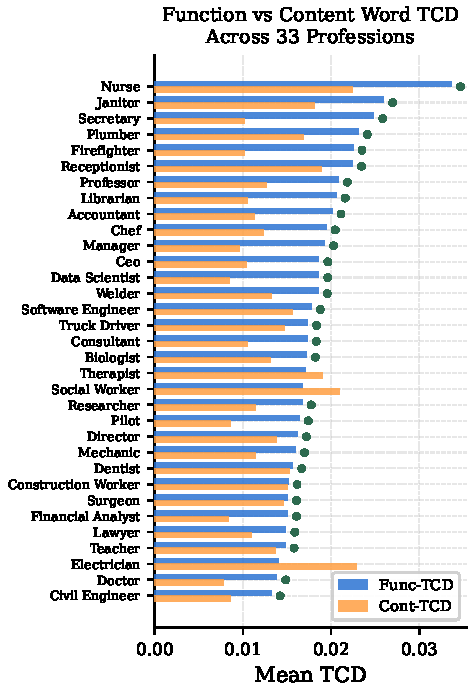
\includegraphics[width=\columnwidth]{figures/func_vs_cont_professions.pdf}
  \caption{Func-TCD (blue) vs.\ Cont-TCD (orange) across 33 professions sorted by Func-TCD. Green dots mark professions where function words carry more bias (30 of 33).}
  \label{fig:func_vs_cont}
\end{figure}

\begin{figure}[t]
  \centering
  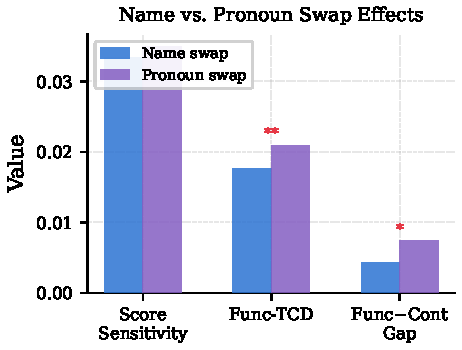
\includegraphics[width=\columnwidth]{figures/name_vs_pronoun.pdf}
  \caption{Comparison of name and pronoun swap effects. Pronoun swaps produce significantly higher Func-TCD ($p = 0.003$, **) and Func$-$Cont gap ($p = 0.017$, *) than name swaps.}
  \label{fig:name_vs_pronoun}
\end{figure}

\paragraph{Mechanism.} BERT's self-attention recomputes all token embeddings when any input changes. Content words (``clinical,'' ``experience'') have strong semantic anchors and shift little; function words (``is,'' ``a'') have weak intrinsic semantics and are almost entirely context-determined. We confirm this via direct measurement: function-word embeddings shift \textbf{8.9$\times$} more than content-word embeddings after an identity swap ($p = 0.0002$).


% ------- 4.2 Rarity Amplification -------
\subsection{Rarity Amplification}
\label{sec:results:rarity}

Names that are rare within the training corpus undergo more BPE fragmentation---e.g., ``Thiruvengadam'' becomes five subword tokens while ``Emily'' remains one. We find that rarity amplifies both Score Sensitivity and Func-TCD:

\begin{table}[t]
\centering
\small
\begin{tabular}{lccc}
\toprule
Name-pair rarity & Mean SS & Mean Func-TCD & Ratio \\
\midrule
Common--Common & 0.0210 & 0.0108 & 1.0$\times$ \\
Common--Rare   & 0.0305 & 0.0163 & 1.5$\times$ \\
\textbf{Rare--Rare}     & \textbf{0.0366} & \textbf{0.0199} & \textbf{1.84$\times$} \\
\bottomrule
\end{tabular}
\caption{Rarity amplification: rare name pairs (more BPE tokens) produce 1.84$\times$ more bias in Func-TCD relative to common pairs. Both profession ($F = 214$, $p < 0.0001$) and rarity ($F = 300$, $p < 0.0001$) are highly significant predictors in ANOVA.}
\label{tab:rarity}
\end{table}

This reveals BPE tokenization as a \emph{hidden fairness tax}: minority-group names are disproportionately fragmented, and fragmentation increases the model's reliance on contextual (bias-laden) representations to process the name. Figure~\ref{fig:rarity} visualizes this stepwise amplification.

\begin{figure}[t]
  \centering
  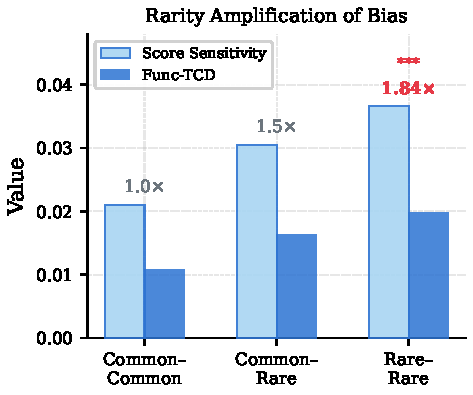
\includegraphics[width=\columnwidth]{figures/rarity_amplification.pdf}
  \caption{Rarity amplification: rare name pairs produce progressively more bias. Rare--Rare pairs show 1.84$\times$ higher Func-TCD than Common--Common pairs ($p < 0.0001$, ***).}
  \label{fig:rarity}
\end{figure}


% ------- 4.3 Name Confound Decomposition -------
\subsection{Confound Decomposition}
\label{sec:results:decomposition}

A name swap simultaneously varies race coding, gender associations, frequency, and tokenization. Using the matched-pair family design (Section~\ref{sec:method:names}), we isolate each factor:

\begin{table}[t]
\centering
\small
\begin{tabular}{lrrcr}
\toprule
Factor & Pairs & SS coef & Func-TCD coef & Func-TCD $p$ \\
\midrule
\textbf{Gender}     & 107 & +0.0088 & \textbf{+0.0049} & $4.5 \times 10^{-9}$ \\
\textbf{Tokenization} & 103 & +0.0067 & \textbf{+0.0048} & $5.3 \times 10^{-4}$ \\
\textbf{Race}       & 124 & +0.0043 & +0.0026           & $4.9 \times 10^{-3}$ \\
Frequency gap       & 100 & +0.0015 & +0.0008           & 0.383 \\
Absolute rarity     & 28  & +0.0024 & +0.0032           & 0.084 \\
\bottomrule
\end{tabular}
\caption{P2b Rosenman-backed targeted validation. Coefficients from OLS with pair-clustered SEs and profession/template fixed effects. Gender and tokenization are the strongest stable signals; race is weaker but detectable; frequency gap is not significant.}
\label{tab:decomposition}
\end{table}

The key interpretation is that name-swap bias is a \textbf{composite effect}: it is not reducible to race alone. Cross-gender contrast and tokenization mismatch are the strongest drivers. A residual race-category signal is detectable but should not be overstated, as it weakens under richer specifications.

In a nested model ladder (P2 full-spec), adding gender to a race-only model increases $R^2$ from 0.157 to 0.183 ($\Delta R^2 = 0.027$), while adding tokenization/frequency further improves to $R^2 = 0.203$. Cross-race weakens rather than strengthens as the specification becomes more realistic. Figures~\ref{fig:decomposition} and~\ref{fig:model_ladder} visualize these patterns.

\begin{figure}[t]
  \centering
  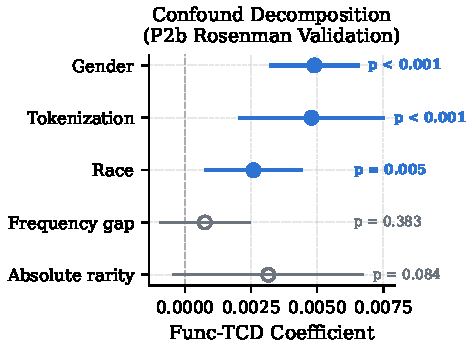
\includegraphics[width=\columnwidth]{figures/decomposition_forest.pdf}
  \caption{Forest plot of Func-TCD coefficients from P2b Rosenman validation. Gender and tokenization are the strongest significant drivers; absolute rarity trends positive but is underpowered ($n=28$).}
  \label{fig:decomposition}
\end{figure}

\begin{figure}[t]
  \centering
  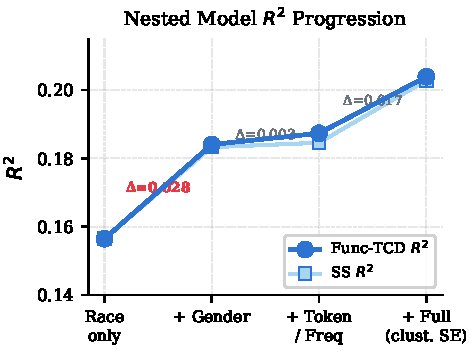
\includegraphics[width=\columnwidth]{figures/model_ladder.pdf}
  \caption{Nested model $R^2$ progression. Adding gender to a race-only model produces the largest $R^2$ jump ($\Delta = 0.028$); cross-race weakens under richer specification.}
  \label{fig:model_ladder}
\end{figure}


% ------- 4.4 Ecological Validation -------
\subsection{Ecological Validation and Cross-Model Comparison}
\label{sec:results:validation}

\paragraph{Real-text generalization.} 
To test whether the function-word effect survives outside synthetic templates, we construct 12 naturalistic passages spanning seven text categories (news, professional biography, legal testimony, medical notes, education reports, letters of recommendation, and community descriptions). Each passage is tested with 10 queries and 14 name pairs (1{,}680 total comparisons).

\begin{table}[t]
\centering
\small
\begin{tabular}{lcccc}
\toprule
Setting & Func-TCD & Cont-TCD & Ratio & $p$ \\
\midrule
Synthetic templates & 0.0177 & 0.0133 & 1.44$\times$ & $2.2 \times 10^{-47}$ \\
\textbf{Natural text} & \textbf{0.0124} & \textbf{0.0087} & \textbf{1.42$\times$} & $\mathbf{6.4 \times 10^{-26}}$ \\
BM25 baseline       & 0.0000 & 0.0000 & ---           & --- \\
\bottomrule
\end{tabular}
\caption{Function-word bias propagation across settings. The ratio is nearly identical between synthetic and natural text (1.44$\times$ vs.\ 1.42$\times$). BM25 produces zero function-word TCD, confirming the effect is specific to contextual models.}
\label{tab:validation}
\end{table}

The function-word dominance pattern is remarkably consistent: \textbf{1.42$\times$} in natural text vs.\ \textbf{1.44$\times$} in synthetic templates, with the natural-text result reaching extreme significance ($t = 10.7$, $p = 6.4 \times 10^{-26}$). The pattern holds across all seven text categories (Figure~\ref{fig:validation}B), with the func$>$cont win rate exceeding 50\% in 9 of 12 individual passages.

\begin{figure*}[t]
  \centering
  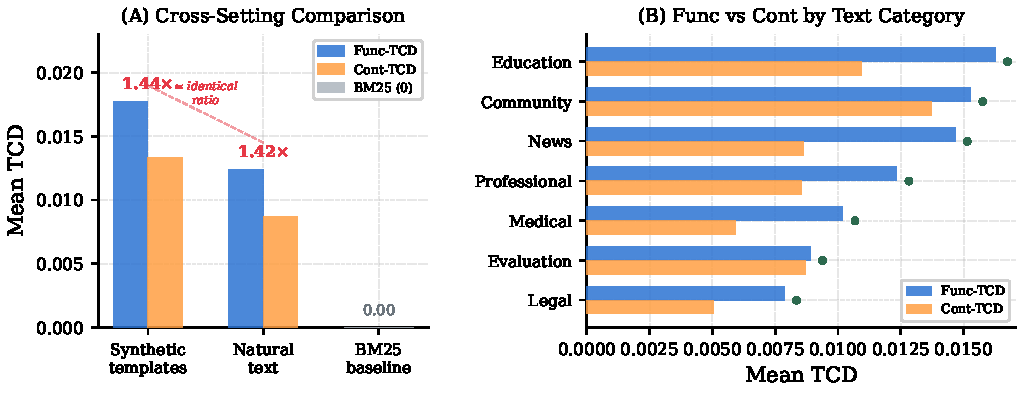
\includegraphics[width=\textwidth]{figures/cross_setting_validation.pdf}
  \caption{Ecological validation. (A)~Cross-setting comparison: the Func/Cont ratio is nearly identical between synthetic templates (1.44$\times$) and natural text (1.42$\times$); BM25 produces zero TCD. (B)~Per-category breakdown of Func-TCD vs.\ Cont-TCD across seven text categories, confirming the pattern generalizes to all categories.}
  \label{fig:validation}
\end{figure*}

\paragraph{BM25 control.}
BM25~\cite{robertson2009} uses exact lexical matching and produces per-term scores that are inherently decomposable. When we apply the same name swaps and compute per-term TCD, we observe \emph{zero} function-word perturbation. This is expected: BM25 scores depend solely on term frequency and IDF, so changing a name only affects the name token's contribution. The result confirms that the ColBERT effect is a consequence of \textbf{contextual representations}, not of retrieval decomposition itself.


% ===========================================================================
\section{Discussion}
\label{sec:discussion}

\subsection{Bias as Distributed Phenomenon}

Our central finding challenges the dominant framing of bias in NLP systems. Traditional bias narratives assume lexical association: ``nurse'' $\leftrightarrow$ ``female'' in the embedding space~\cite{bolukbasi2016, caliskan2017}. In contextual retrieval models, bias is instead \emph{distributed}: it propagates through self-attention into tokens that have no semantic relationship with the identity being tested. The ``is'' in ``Lakisha is an experienced doctor'' encodes identity information not because ``is'' has any intrinsic gender or racial meaning, but because BERT's attention mechanism makes function-word representations exquisitely sensitive to context.

\subsection{Tokenization as Infrastructure-Level Bias}

The rarity amplification finding (Section~\ref{sec:results:rarity}) identifies BPE tokenization as a structural bias amplifier. Names common in majority populations (``Emily,'' ``Greg'') tend to survive as single tokens, while names from minority groups (``Lakisha,'' ``Thiruvengadam'') are fragmented into multiple subword pieces. This fragmentation forces the model to ``assemble'' the name from parts, increasing uncertainty and amplifying reliance on stereotyped contextual priors. The result is a \emph{hidden tax}: the same document about the same profession receives different retrieval treatment depending on how ``expensive'' the name is to tokenize.

This finding complements and extends recent work connecting tokenization disparities to downstream fairness harms in other settings. Ovalle et al.~(\citeyear{ovalle2024}) demonstrated that BPE over-fragmentation of neopronouns directly causes LLM misgendering, and proposed ``pronoun tokenization parity'' as a mitigation. Petrov et al.~(\citeyear{petrov2023}) showed that multilingual tokenizers introduce systematic cost unfairness across languages. Our contribution is to establish the same causal pathway---fragmentation $\to$ bias amplification---in the retrieval domain, and to quantify it at the individual token level via TCD. Together, these findings suggest that BPE tokenization is not merely a performance bottleneck but an \emph{active fairness hazard} that operates across generation, retrieval, and cross-lingual settings.

\subsection{ColBERT as a Diagnostic Instrument}

An important implication of our findings is that ColBERT is not simply a retrieval model---it is a \textbf{diagnostic instrument} for contextual bias. Single-vector models (DPR, ANCE) may exhibit the same or worse bias, but because they collapse all tokens into one embedding, there is no way to ask \emph{which token caused the score difference}. ColBERT's late interaction makes the internal structure of bias visible. This parallels the role of medical imaging: an X-ray does not make you sick, but it lets you see where the disease is.

\subsection{Implications for Debiasing}

Traditional debiasing methods---gender-direction removal~\cite{bolukbasi2016}, adversarial training~\cite{rekabsaz2021}---target specific word embeddings or aggregate representations. Our finding that bias concentrates in function words suggests a more targeted intervention: \emph{function-word-specific null-space projection}. By collecting the embedding-difference vectors of function words across counterfactual pairs and projecting function-word representations onto the orthogonal complement of the identity-sensitive subspace, one could remove identity information from the tokens that carry the most bias while leaving content-word representations intact. We leave empirical validation of this approach to future work.


% ===========================================================================
\section{Limitations}
\label{sec:limitations}

\paragraph{Synthetic and semi-synthetic data.} While we validate on naturalistic passages (Section~\ref{sec:results:validation}), our primary analyses use template-generated counterfactual pairs. A full MS~MARCO evaluation with NER-based name extraction would strengthen ecological validity.

\paragraph{Single model.} We tested only ColBERTv2. While the BM25 control confirms contextual specificity, comparison with other dense retrievers (DPR, SPLADE) is needed.

\paragraph{Name pool scope.} Our 65-name pool covers four US-centric racial categories (White, Black, Hispanic, Asian). Names from other geographies and ethnicities are not represented.

\paragraph{Absolute rarity.} The absolute\_rarity factor reaches marginal significance ($p = 0.084$) with 28 pairs. A larger name expansion is needed to resolve this mechanism.

\paragraph{No debiasing evaluation.} We identify the mechanism but do not implement or evaluate mitigation. The null-space projection proposal remains theoretical.


% ===========================================================================
\section{Conclusion}
\label{sec:conclusion}

We have shown that identity-related bias in ColBERT does not reside where intuition suggests. It is not the word ``doctor'' or ``nurse'' that carries bias into the retrieval score---it is the word ``is.'' This distributed, context-mediated propagation through function words is (1)~robust across 33 professions, (2)~amplified by BPE tokenization of rare names, (3)~driven primarily by gender contrast and tokenization mismatch rather than race alone, (4)~replicated at near-identical magnitude in naturalistic text, and (5)~entirely absent in non-contextual retrieval. These findings reframe both the measurement and the mitigation of bias in neural retrieval systems: bias is not a localized pathology but a systemic property of contextual representations.


% ===========================================================================
\begin{acks}
This work was conducted as part of CSCI~2952W at Brown University. The Rosenman et al.\ first-name ethnicity data was obtained from the Harvard Dataverse (DOI: 10.7910/DVN/SGKW0K).
\end{acks}


\bibliographystyle{ACM-Reference-Format}
\bibliography{refs}

\end{document}
